% Supplementary Figure S1 (combined): S1 serpentine layout with chemostat diagrams inside each step box.
\def\SimLoopColW{5.45cm}
\def\SimLoopGap{1.05cm}
\def\SimLoopSpan{11.95cm} % 2 * \SimLoopColW + \SimLoopGap
\def\SimLoopInitGap{0.55cm}
\def\SimLoopComboLoopDrop{1.15cm} % init bottom -> loop top (room for genlabel)
\def\SimLoopComboGap{0.32cm}
\def\SimLoopOutcomeGap{1.5cm}
\def\SimLoopOutcomeWide{6.85cm}
\def\SimLoopCollapseNarrow{4.25cm}
\def\SimLoopComboSnapW{4.25cm}
\def\SimLoopComboSnapSpanW{5.05cm}

% Pre-rendered PDFs (scripts/build_chemostat_snapshot_pdfs.sh) avoid nested-TikZ distortion.
\newcommand{\SimLoopComboSnap}[1]{%
  \\[4pt]%
  \includegraphics[width=\SimLoopComboSnapW]{chemostat_snap/#1.pdf}%
}
\newcommand{\SimLoopComboSnapSpan}[1]{%
  \\[4pt]%
  \includegraphics[width=\SimLoopComboSnapSpanW]{chemostat_snap/#1.pdf}%
}
\newcommand{\SimLoopComboEnergySnap}{%
  \\[4pt]%
  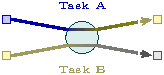
\includegraphics[width=\SimLoopVisEnergyWidthScale\dimexpr\SimLoopComboSnapW\relax]{chemostat_snap/energy_noeq.pdf}%
}

\begin{tikzpicture}[
  font=\small,
  >=Stealth,
  proc/.style={
    draw=blue!70!black, fill=blue!10, rounded corners=3pt,
    align=center, text width=\SimLoopColW, minimum width=\SimLoopColW,
    inner sep=4pt},
  init/.style={
    draw=teal!70!black, fill=teal!10, rounded corners=3pt,
    align=center, text width=\SimLoopSpan, minimum width=\SimLoopSpan,
    inner sep=4pt},
  check/.style={
    draw=yellow!60!black, fill=yellow!18, rounded corners=3pt,
    align=center, text width=\SimLoopSpan, minimum width=\SimLoopSpan,
    inner sep=4pt},
  outcome/.style={
    draw=teal!70!black, fill=teal!10, rounded corners=3pt,
    align=center, inner sep=4pt},
  stop/.style={
    draw=gray!60, fill=gray!8, rounded corners=3pt,
    align=center, font=\footnotesize, inner sep=4pt},
  looplabel/.style={
    draw=gray!55, fill=white, rounded corners=2pt,
    align=center, font=\scriptsize, inner sep=3pt},
  loopbox/.style={
    draw=blue!40!black, rounded corners=5pt, inner sep=8pt},
  orth/.style={thick, -Stealth},
]

\node[init] (init) {%
  \textbf{Initialize Run:} homogeneous genotype $A_0$ with $B_0{=}1{-}A_0$; start population $N_0{=}100$;\\
  fix sampled parameters\SimLoopComboSnapSpan{init}};

\coordinate (L) at ($(init.south west)+(0.5*\SimLoopColW,0)$);
\coordinate (R) at ($(init.south east)+(-0.5*\SimLoopColW,0)$);

\begin{scope}[local bounding box=loopcontent]
  \node[proc, anchor=north] (inflow) at ($(L |- init.south)+(0,-\SimLoopComboLoopDrop)$) {%
    \textbf{1. Resource Inflow}\\
    Add fresh $M_1$ to the well-mixed environment pool\SimLoopComboSnap{inflow}};

  \node[proc, anchor=north] (taskA) at ($(R |- init.south)+(0,-\SimLoopComboLoopDrop)$) {%
    \textbf{2. Task~A}\\
    Convert $M_1 \rightarrow M_2$; task done by organisms according to their $A_i$%
    \SimLoopComboSnap{taskA}};

  \path let \p1=(inflow.south), \p2=(taskA.south) in
    coordinate (rowonebot) at (0, {min(\y1,\y2)});

  \node[proc, anchor=north] (energy) at ($(L |- rowonebot)+(0,-\SimLoopComboGap)$) {%
    \textbf{4. Energy Accounting}\\
    Credit Task~A and Task~B yields to $E_i^{(g-1)}$, then deduct maintenance $c_{\mathrm{m}}$:\\
    $E_i^{(g)} \leftarrow E_i^{(g-1)} + \mathcal{A}_i + Y\cdot\mathcal{B}_i - c_{\mathrm{m}}$%
    \SimLoopComboEnergySnap};

  \node[proc, anchor=north] (taskB) at ($(R |- rowonebot)+(0,-\SimLoopComboGap)$) {%
    \textbf{3. Task~B}\\
    Convert $M_2 \rightarrow$ waste; task done by organisms according to their $B_i$%
    \SimLoopComboSnap{taskB}};

  \path let \p1=(energy.south), \p2=(taskB.south) in
    coordinate (rowtwobot) at (0, {min(\y1,\y2)});

  \node[proc, anchor=north] (death) at ($(L |- rowtwobot)+(0,-\SimLoopComboGap)$) {%
    \textbf{5. Death}\\
    Draw $P_{\mathrm{death},i}(E_i)$ for each organism; remove dead organisms%
    \SimLoopComboSnap{death}};

  \node[proc, anchor=north] (dup) at ($(R |- rowtwobot)+(0,-\SimLoopComboGap)$) {%
    \textbf{6. Reproduction}\\
    Draw $P_{\mathrm{repro},i}(E_i)$ for each organism; split energy between parent and offspring;\\
    offspring receives a copy of the parent's traits ($A_i$, $B_i$)\SimLoopComboSnap{dup}};

  \path let \p1=(death.south), \p2=(dup.south) in
    coordinate (rowthreebot) at (0, {min(\y1,\y2)});

  \node[proc, anchor=north] (flow) at ($(L |- rowthreebot)+(0,-\SimLoopComboGap)$) {%
    \textbf{8. Chemostat Flow}\\
    Draw $P(\mathrm{outflow}_i)$ for each survivor; remove organisms and\\
    scale environmental $M_1$ \& $M_2$ by $(1-\phi)$\SimLoopComboSnap{outflow}};

  \node[proc, anchor=north] (mutate) at ($(R |- rowthreebot)+(0,-\SimLoopComboGap)$) {%
    \textbf{7. Trait Mutation}\\
    With probability $\mu_{\mathrm{m}}$, modify offspring traits within $\pm\sigma_{\mathrm{m}}$\\
    of the parental value; see Supplementary Methods%
    \SimLoopComboSnap{mut}};

  \coordinate (linkA) at (inflow.east |- taskA.west);
  \coordinate (link34) at (taskB.west |- energy.east);
  \coordinate (link56) at (death.east |- dup.west);
  \coordinate (link78) at (mutate.west |- flow.east);
  \draw[orth] (linkA) -- (taskA.west);
  \draw[orth] (taskA.south) -- (taskB.north);
  \draw[orth] (link34) -- (energy.east);
  \draw[orth] (energy.south) -- (death.north);
  \draw[orth] (link56) -- (dup.west);
  \draw[orth] (dup.south) -- (mutate.north);
  \draw[orth] (link78) -- (flow.east);
\end{scope}

\node[loopbox, fit=(loopcontent)] (loopframe) {};
\node[font=\footnotesize\bfseries, anchor=south east, inner sep=2pt] (genlabel)
  at (loopframe.north east) {For each generation~-- $g = 1,\ldots,1{,}000$};

\node[check, below=\SimLoopComboLoopDrop of loopframe.south] (check) {%
  \textbf{9. End of Generation}\SimLoopComboSnapSpan{endgen}};

\node[font=\footnotesize, anchor=south east, inner sep=2pt, align=right] (nglabel)
  at (check.north east)
  {$N_g$ -- final population size at generation~$g$};

\coordinate (outrow) at ($(check.south)+(0,-\SimLoopOutcomeGap)$);

\node[outcome, anchor=north west, text width=\SimLoopOutcomeWide,
  minimum width=\SimLoopOutcomeWide] (analyze) at ($(init.south west |- outrow)$) {%
  \textbf{10. Cross-Feeding Outcome Analysis}\\
  Evaluate the final population for persistence, specialization, and deviation from neutral drift (Methods);\\
  record hit/non-hit\SimLoopComboSnap{score}};

\node[stop, anchor=north east, text width=\SimLoopCollapseNarrow,
  minimum width=\SimLoopCollapseNarrow] (stoprun) at ($(init.south east |- outrow)$) {%
  \textbf{Run Ends (Collapsed)}\\
  Population extinct before generation 1{,}000; no outcome scoring\SimLoopComboSnap{collapse}};

\coordinate (loopback) at ($(check.west)+(-1.45cm,0)$);
\coordinate (loopup) at (loopback |- inflow.west);

\coordinate (initmid) at ($(init.south)!0.55!(loopframe.north)$);
\draw[orth] (init.south) -- (initmid) -| (inflow.north);
\path let \p1=(flow.south), \p2=(check.north) in
  coordinate (flowvcorner) at (\x1, {0.5*\y1+0.5*\y2})
  coordinate (flowhcorner) at (\x2, {0.5*\y1+0.5*\y2});
\draw[orth] (flow.south) -- (flowvcorner) -- (flowhcorner) -- (check.north);
\coordinate (checkL) at ($(analyze.north |- check.south)$);
\coordinate (checkR) at ($(stoprun.north |- check.south)$);
\draw[orth] (checkL) -- node[midway, looplabel] {$g = 1{,}000$,\\$N_g > 0$} (analyze.north);
\draw[orth] (checkR) -- node[midway, looplabel] {$N_g = 0$} (stoprun.north);
\draw[orth] (check.west) -- (loopback)
  -- node[midway, looplabel] {$g < 1{,}000$,\\$N_g > 0$} (loopup)
  -- (inflow.west);

% Legend in the same TikZ picture (avoid nested-TikZ). Fit both outcome boxes so
% the taller score panel stays inside the TeX bounding box.
\ChemostatSnapStyles
\node[fit=(analyze)(stoprun), inner sep=0pt, draw=none] (outcomefit) {};
\matrix[
  column sep=0.35cm,
  ampersand replacement=\&,
  nodes={inner sep=0pt, anchor=base},
  row sep=0pt,
  anchor=north,
] (simlegend) at ($(outcomefit.south)+(0,-0.55cm)$) {
  \node[csmballMone] {}; \&
  \node[font=\scriptsize] {$M_1$}; \&
  \node[csmballMtwo] {}; \&
  \node[font=\scriptsize] {$M_2$}; \&
  \node[csmballWaste] {}; \&
  \node[font=\scriptsize] {Waste}; \&
  \node[csorg] {}; \&
  \node[font=\scriptsize] {Organism}; \&
  \node[csorgMut] {}; \&
  \node[font=\scriptsize] {Mutant offspring}; \\
};

\coordinate (bboxSouth) at ($(simlegend.south)+(0,-0.25cm)$);

\pgfresetboundingbox
\useasboundingbox
  ([xshift=-1.65cm,yshift=4pt]init.north west)
  rectangle
  ([xshift=1.65cm]init.east |- bboxSouth);

\end{tikzpicture}
